\includepdf[pages=2]{Quiz1.pdf}

\begin{figure}[H]
    \centering
    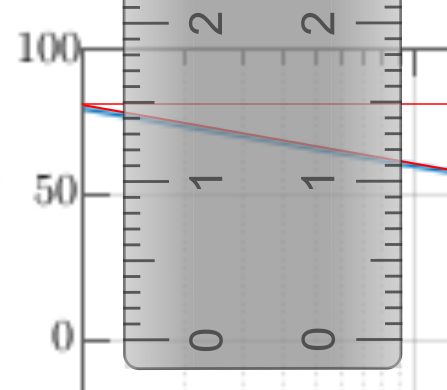
\includegraphics[width=0.3\textwidth]{imagenes/medicion_inicio.png}
    \caption{
        Medición de ganancia inicial del diagrama de bode
    }\label{inicio}
\end{figure}

En la figura~\ref{inicio} se tienen las siguientes mediciones \\ \\
Medición de referencia: $50\,dB = 0{.}9\,\mathrm{u}$ \\
Medición de objetivo: $x\,dB = 1{.}5\,\mathrm{u}$

\begin{equation*}
    \dfrac{x}{1{.}5} = \dfrac{50}{0{.}9} \Longrightarrow
     x = \dfrac{50 \cdot 1{.}5}{0{.}9} = 83{.}33 \, dB
\end{equation*}

\begin{figure}[H]
    \centering
    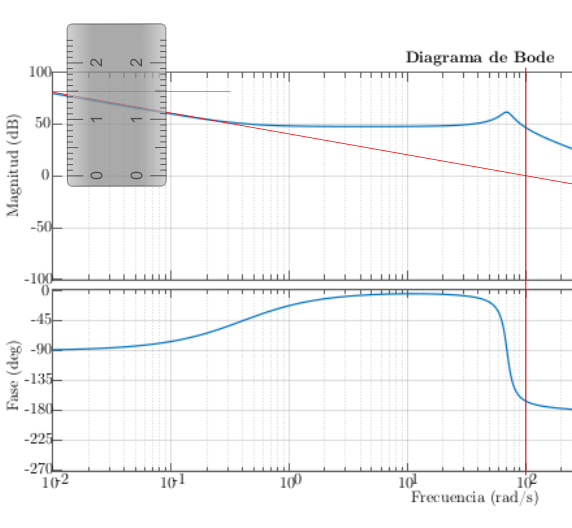
\includegraphics[width=0.5\textwidth]{imagenes/medicion_pendiente.png}
    \caption{
        Medición de pendiente del diagrama de bode
    }\label{fig:pendiente}
\end{figure}

Se puede notar que desde el inicio del diagrama de bode hasta que llega a 0 dB
pasan 4 decadas por lo que se esa pendiente es de $-20{.}83\,dB$ por decada.
Por lo que aproximaremos a decir que esta pendiente es $-20\,dB$ por decada. \\

Como la fase empieza en $-90^\mathrm{o}$ y la pendiente inicial 
es de $-20\,dB$ por decada por lo qué la función de transferencia tiene
un polo $s^{-1}$

Una forma tentativa para la función de transferencia es la siguiente:

\begin{equation*}
    H(s) = \dfrac{K}{s} \cdot \dfrac{A(s)}{B(s)}
\end{equation*}

Puesto que debe tener minimo un cero, ya que la función tiene ganancia
constante en un rango, por lo que debe en dicho rango cancelar el polo $s^{-1}$
\\

\begin{figure}[H]
    \centering
    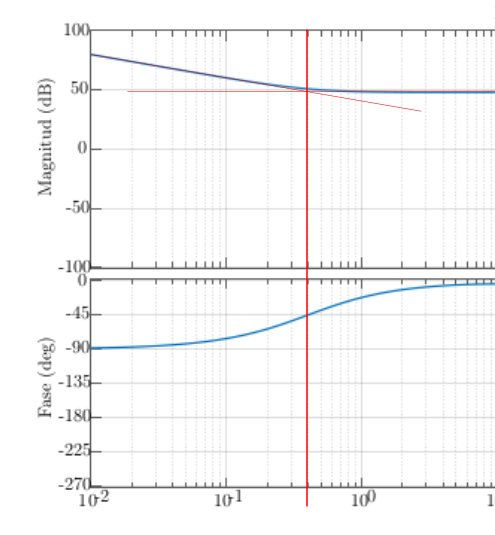
\includegraphics[width=0.4\textwidth]{imagenes/esquina_cero.png}
    \caption{
        Medición de frecuencia de esquina de cero del diagrama de bode
    }\label{fig:cero}
\end{figure}

Este cero empieza a partir de $4\times 10^{-1} \, \frac{rad}{s}$

Actualizando la función de transferencia:
\begin{equation*}
    H(s) = \dfrac{K}{s} \cdot \dfrac{\frac{s}{0{.}4} + 1}{B(s)}
\end{equation*}

Ahora faltan los polos, se puede notar que existe un pico de resonancia
positivo, por lo que la función de transferencia tiene un polo cuadrático.

Dicho pico de resonancia está situado en $7\times 10^{1} \, \frac{rad}{s}$

\begin{figure}[H]
    \centering
    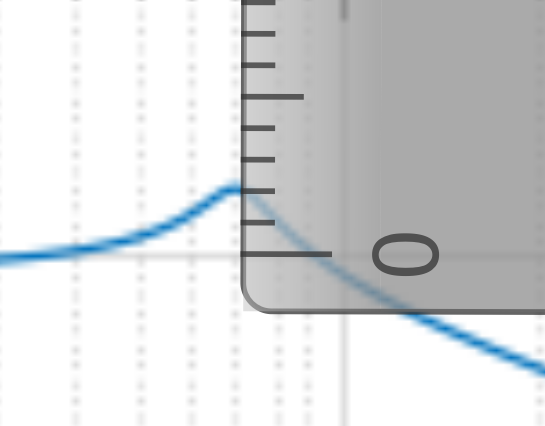
\includegraphics[width=0.3\textwidth]{imagenes/medicion_mr.png}
    \caption{
        Medición del pico de sobre paso del diagrama de bode
    }\label{fig:mp}
\end{figure}

Volvemos a usar la medición de referencia de la figura~\ref{inicio} \\ \\
Medición de referencia: $50\,dB = 0{.}9\,\mathrm{u}$ \\
Medición de objetivo: $x\,dB = 0{.}2\,\mathrm{u}$

\begin{equation*}
    \dfrac{x}{0{.}2} = \dfrac{50}{0{.}9} \Longrightarrow
     x = \dfrac{50 \cdot 0{.}2}{0{.}9} \approx 11 \, dB
\end{equation*} 

\vspace{1cm}

Usando la ecuación que nos entrega la longitud del pico de resonancia, podemos
obtener $\xi$

\begin{equation*}
    M_{p(dB)} = 20 \log_{10}
    {\left({\left(
         2\xi{\sqrt{1 - \xi^2}}
    \right)}^{-1}\right) }
\end{equation*}

\begin{multicols}{2}

\begin{equation*}
    20 \log_{10}
    {\left({\left(
         2\xi{\sqrt{1 - \xi^2}}
    \right)}
    \right)}  = {-1} \cdot 11 \, dB
\end{equation*}
\begin{equation*}
    \log_{10}
    \left(
         2\xi{\sqrt{1 - \xi^2}}
    \right)  =  \frac{-11}{20}
\end{equation*}
\begin{equation*}
        2\xi{\sqrt{1 - \xi^2}}
    =  10^{\frac{-11}{20}}
\end{equation*}

\begin{equation*}
    4\xi^2
    \left(   
    {1 - \xi^2}
    \right)
    =  10^{\frac{-22}{20}}
\end{equation*}

\begin{equation*}
    4\xi^2
    -4\xi^4
    -10^{\frac{-22}{20}}
    =  0
\end{equation*}

\begin{equation*}
    \xi_1 = 0{.}98981
\end{equation*}
\begin{equation*}
    \xi_2 = 0{.}14237
\end{equation*}
\begin{equation*}
    \xi_3 = -0{.}14237
\end{equation*}
\begin{equation*}
    \xi_4 = -0{.}98981
\end{equation*}

\end{multicols}

$\xi$ debe ser un valor entre 0 y 0.707 para que la ecuación de $M_p$
tenga validez, el unico resultado que cumple esta condición es 
$\xi = 0{.}14237$ \\

Ahora para obtener $\omega_n$:

\begin{equation*}
    7\times 10^{1} \, \frac{rad}{s} = \omega_n \sqrt{1 - 2{(0{.}14237)}^2}
\end{equation*}

por lo que $\omega_n$:

\begin{equation*}
    \omega_n  = \dfrac{70}{\sqrt{1 - 2{(0{.}14237)}^2}} = 71{.}46
\end{equation*}

por lo que la expresión de esta función cuadrática deberá ser:

\begin{equation*}
\dfrac{s^2}{71{.}46^2} + 2\cdot 0{.}14237 \cdot \dfrac{s}{71{.}46} + 1 
\end{equation*}

Actualizando la función de transferencia:
\begin{equation*}
    H(s) = \dfrac{K}{s} \cdot \dfrac{\frac{s}{0{.}4} + 1}{
        \left(
            \dfrac{s^2}{71{.}46^2} 
            + 2\cdot 0{.}14237 \cdot
            \dfrac{s}{71{.}46} + 1 
        \right) \cdot C(s)
        }
\end{equation*}

Se sabe que hace falta un polo

Debido a que el diagrama de fase empieza en $-90^{\mathrm{o}}$ y termina en 
$-270^{\mathrm{o}}$.

\begin{itemize}
\item polo $s^{-1}$ aporta $-90^{\mathrm{o}}$ 
\item polo cuadrático aporta $-180^{\mathrm{o}}$ 
\item cero ${(\frac{s}{0{.}4} + 1)}$ aporta $90^{\mathrm{o}}$
\end{itemize}

Por lo que faltan $-90^{\mathrm{o}}$ para llegar a $-270^{\mathrm{o}}$ en el
diagrama de fase, siendo esta la razón por la que se concluyó que hacia falta
un polo. 

\begin{figure}[H]
    \centering
    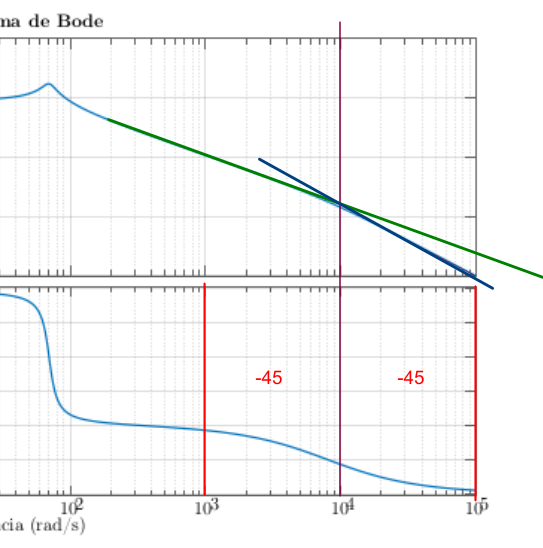
\includegraphics[width=0.5\textwidth]{imagenes/ultimo_polo.png}
    \caption{
        Medición para encontrar último polo
    }\label{fig:ult_polo}
\end{figure}

Tanto el diagrama de fase como el diagrama de ganancia indican 
que la frecuencia de esquina es $10^{4} \, \frac{rad}{s}$

Actualizando la función de transferencia:
\begin{equation*}
    H(s) = \dfrac{K}{s} \cdot \dfrac{\frac{s}{0{.}4} + 1}{
        \left(
            \dfrac{s^2}{71{.}46^2} 
            + 2\cdot 0{.}14237 \cdot \dfrac{s}{71{.}46} + 1 
        \right) \cdot (\frac{s}{10^4} + 1)
        }
\end{equation*}


Ahora debemos proceder a obtener K\@: \\

\newcommand{\frecuencia}{1}
\newcommand{\ganancia}{50}

Se sabe que la ganancia en {\frecuencia} $\frac{rad}{s}$ es de {\ganancia} dB
 \\

Pasamos el aporte de los ceros y polos en ${\frecuencia} \frac{rad}{s}$ a dB

\begin{equation*}
    20\log_{10}(K)
\end{equation*}

\begin{equation*}
     20\log_{10}\sqrt{1 + {(\frac{\frecuencia}{0{.}4})}^2}
     = 8{.}60\,\,_{dB} 
\end{equation*}

\begin{equation*}
    -20\log_{10}
    \left(
        \frac{1}{{\frecuencia}}
    \right) = 0
\end{equation*}


\begin{equation*}
     -20\log_{10}\sqrt{1 + {(\frac{\frecuencia}{10^4})}^2}
     = -4{.}34\times 10^{-8}\,\,_{dB} 
\end{equation*}

\begin{equation*}
    -20\log_{10}\sqrt{{\left(1-{(\frac{\frecuencia}{71{.}46})}^2\right)}^2 
    + {\left(2 \cdot 0{.}14237 \cdot \frac{\frecuencia}{71{.}46} \right)}^2}
    = 1{.}6321 \times 10^{-3}\,\,_{dB} 
\end{equation*}

Igualamos la ganancia {\ganancia} con las ganancias obtenidas

\begin{equation*}
    \ganancia = 20\log_{10}(K) 
    + 8{.}60 
    + 0 
    - 4{.}34\times 10^{-8} 
    + 1{.}6321 \times 10^{-3}
\end{equation*}

\begin{equation*}
    41{.}4 = 20\log_{10}(K)   
\end{equation*}

Por lo que K es:

\begin{equation*}
    K = 10 ^{\frac{41{.}4}{20}}  \approx 117{.}5
\end{equation*}

Finalmente la función de transferencia es\@: 

\begin{equation*}
    H(s) = \dfrac{117{.}5}{s} \cdot \dfrac{\frac{s}{0{.}4} + 1}{
        \left(
            \dfrac{s^2}{71{.}46^2} 
            + 2\cdot 0{.}14237 \cdot \dfrac{s}{71{.}46} + 1 
        \right) \cdot (\frac{s}{10^4} + 1)
        }
\end{equation*}